\section{d1: Adapting Pre-trained Masked dLLMs to Reasoning Models}


We propose d1, a two-stage framework that enhances the reasoning performance of pre-trained masked dLLMs by sequentially combining SFT and online RL. \looseness=-1


Online RL, particularly the GRPO algorithm,  has demonstrated its efficacy in improving the performance of offline trained language model~\citep{shao2024deepseekmath, guo2025deepseek, team2025kimi}. 
However, the learning formulation of GRPO does not directly generalize to dLLMs. The objective of GRPO \eqref{eq:grpo_loss} requires computing the (log-)likelihood ratio of $\pi_\theta$ and $\pi_{\theta_{\text{old}}}$, at both the token level (for the advantage weights) and the sequence level (for the reverse KL term). \hl{Generally speaking, we need to efficiently compute the per-token and the sequence log-probability of dLLMs' completion $o$.} Autoregressive~(AR) models, such as Transformers, directly model the per-token log-probabilities, and the sequence-level log-probability of $o$ can be easily computed through the chain rule using one forward pass:
$\log \pi_\text{AR}(o|q) = \sum_{k=1}^{|o|} \log \pi_\text{AR}(o^k|q, o^{<k})$. Similarly, the KL term can be decomposed as
$
D_{\text{KL}}\left[\pi_\theta(\cdot | q)\| \pi_\text{ref}(\cdot | q) \right] = \E_{o \sim \pi_\theta(\cdot \mid q)} \left[ \sum_{k=1}^{|o_i|} \log \frac{\pi_\theta(o^k|q, o^{<k})}{\piref(o^k|q, o^{<k})}   \right]
$. Unlike AR models, dLLMs do not adhere to sequential factorization of the sequence log-probability. Meanwhile, the per-token log-probability are also costly to compute since the decoding process invokes the unmasking predictor $f_\theta$ multiple times\footnote{In other words, $\pi_\theta$ is a composition of $M$ $f_\theta$ functions for a $M$-step decoding process}. As the first step, we propose an efficient log-probability estimator in \cref{sec:method_logprob}. Next, using these estimators, we introduce \grpo, a variant of GRPO for dLLMs in \cref{sec:method_grpo}. Last, we discuss our SFT recipe in \cref{sec:method_sft}.


\vspace{-2mm}
\subsection{Efficient Log Probability Estimation for Masked dLLMs}
\label{sec:method_logprob}
\vspace{-1.6mm}

For sequence log-probability, we use a mean-field approximation that decomposes it into a product of independent per-token log-probabilities.
For per-token log-probability, we introduce an estimation method that only calls $f_\theta$ once.

\textbf{Mean-Field Approximation of Sequence Log Probability.} 
As opposed to AR models, dLLMs treat the token sequence as a whole and therefore its sequence-level log-probability lacks the AR decomposition. 
To efficiently estimate it, we use a simple mean-field decomposition to approximate $\log \pi_\theta(o| q)$ by $\sum_{k=1}^{|o|} \log \pi_\theta(o^k | q)$. The per-token log-probability estimation is introduced below.

\textbf{One-Step Per-Token Log Probability Estimation with Prompt Masking.} 
Let $\oplus$ denote the concatenation operator. Given a prompt $q$, the decoding process starts from an initial sequence $q \oplus \mask \oplus \ldots \oplus \mask$ (up to a preset length). To compute the log-probability of $o$, we perturb $q$ where every token is randomly masked out with probability $p_{\text{mask}}$, resulting in a new prompt $q'$. We then do one-step unmasking to obtain $\log f_\theta( o^k | q' \oplus \mask  \ldots \oplus \mask )$ and use it as an estimation of $\log \pi_\theta(o^k | q)$, $1\leq k \leq |o|$.  We discuss the motivation of using a masked prompt $q'$ in the next section. \looseness=-1

\begin{figure}[t]
    \centering
    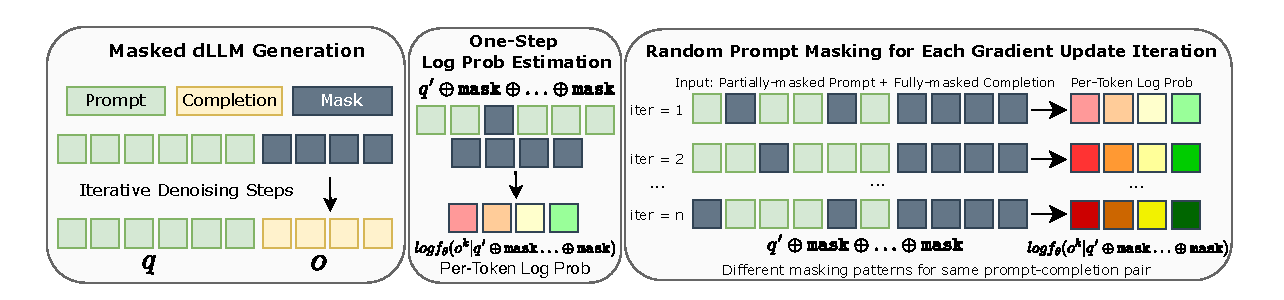
\includegraphics[width=\columnwidth]{figs/diffugrpo.pdf}
    \caption{\textbf{Log Probability Estimation in \grpo{}.} After generating completion $o$ from prompt $q$ using full diffusion denoising (left), we compute token-level log probabilities with a single forward pass per masking pattern (mid) and use the log-probability of one-step unmasking as our estimation. During each policy gradient update, we apply a random masking pattern to the prompt, creating $q'$, while keeping the completion fully masked (right). The gradient of colors in the per-token log probabilities demonstrates that each distinct masking pattern yields a different estimate of the per-token log probabilities. This serves as a form of regularization for policy optimization, allowing more gradient updates per batch and thereby reducing the number of online generations needed for RL training. \looseness=-1
    }
\label{fig:log_prob_estimation}
\end{figure}
We note that LLaDA~\citep[Algorithm 3]{nie2025largelanguagediffusionmodels} uses a Monte Carlo type of approximation to estimate the log-probabilities, where they use a MC sample size is $128$. This estimator is inefficient for online RL, since it creates a large computational graph with hundreds of forward passes, resulting in inefficient policy optimization and excessive memory usage. 



\subsection{\grpo: Policy Gradient Optimization for Masked dLLMs}
\label{sec:method_grpo}

\begin{algorithm}[t]
\caption{\grpo{}: Policy Gradient Optimization for Masked dLLMs}
\begin{algorithmic}[1]
\Require Reference model $\piref$, prompt distribution $\mathcal{D}$, number of completions per prompt $G$, number of inner updates $\mu$, prompt token masking probability $p_\text{mask}$
    \State Initialize $\pi_{\theta} \gets \piref$
    \While{not converged}
        \State $\piold \gets \pi_{\theta}$
        \State Sample a prompt $q \sim \mathcal{D}$
        \State Sample $G$ completions $o_i \sim \piold(\cdot\mid q)$, $i \in [G]$ 
        \State For each $o_i$, compute reward $r_i$ and advantage $A^k_{i}(\piold)$ using \cref{eq:our_adv}
        \For{gradient update iterations $n = 1, \ldots, \mu$}
            \State $q' \gets$ randomly mask tokens of prompt $p$ with probability $p_\text{mask}$
            \State For $\pi_\theta$, $\piold$, $\piref$, estimate log-probabilities of $o_i$ given $q'$ according to \cref{sec:method_logprob}
            \State Compute \grpo objective \eqref{eq:diffugrpo} and update $\pi_{\theta}$ by gradient descent
        \EndFor
    \EndWhile
\State \Return $\pi_{\theta}$
\end{algorithmic}
\label{algo:grpo}
\end{algorithm}


Using the log-probability estimators proposed in \cref{sec:method_logprob}, we extend GRPO to masked dLLMs. Note that our estimation technique is broadly applicable and can readily extend to other policy gradient methods such as PPO~\citep{schulman2017proximal} or REINFORCE~\citep{williams1992simple}.

Let  $\phi^{\pi_\theta}(o^k \mid q')$ and $\phi^{\pi_\theta}(o \mid q')$  denote the estimated per-token and sequence probabilities for $\pi_\theta$. 
We derive the loss function of \grpo,
\begin{equation}
\resizebox{0.94\columnwidth}{!}{$%
\begin{aligned}
\mathcal{L}_{\text{\grpo{}}}(\theta)=\;&
\E_{\substack{q \sim \mathcal{D},\, q' \sim \text{masking}(q),\\
              o_1,\dots,o_G \sim \piold(\,\cdot \mid q)}}\Bigg[
\frac{1}{G}\sum_{i=1}^{G}\frac{1}{|o_i|}\sum_{k=1}^{|o_i|}
\min\!\Bigg(
      \frac{\phi^{\pi_\theta}(o^k_i \mid q')}
           {\phi^{\piold}(o^k_i \mid q')}A_i^{k},\\[4pt]
&\operatorname{clip}\!\Bigg(
        \frac{\phi^{\pi_\theta}(o^k_i \mid q')}
             {\phi^{\piold}(o^k_i \mid q')},
        1-\varepsilon,\,1+\varepsilon
  \Bigg)A_i^{k}
\Bigg)
-\beta\,D_{\text{KL}}\!\Bigl[
   \phi^{\pi_\theta}(\cdot \mid q')\,\bigl\|\,\phi^{\piref}(\cdot \mid q')
\Bigr]
\Bigg]
\end{aligned}$}%
\label{eq:diffugrpo}
\end{equation}
Our algorithm is summarized in \cref{algo:grpo}.
To efficiently optimize the policy loss, in practice, on-policy RL algorithms such as PPO and GRPO perform multiple gradient updates for each batch of samples. During these updates,  the prompt $q$, completions $\set{o_i}^G_{i=1}$, old policy $\piold$ and advantages $A^k_i(\piold)$ are kept fixed. However, determining the optimal number of gradient updates per batch is challenging. If the number is too high, it can lead to overfitting within the batch, while a number that is too low slows down convergence. Achieving a balance between outer batch iterations and inner gradient updates is crucial for sample efficiency. Besides, every outer batch iteration requires sampling completion through iterative denoising steps, which incurs high computational cost.


Interestingly, our log-probability estimator offers a unique mitigation to this dilemma. For each gradient update step, we randomly mask the prompt $q$ to $q'$
to estimate the log-probabilities. Intuitively, this stochastic masking introduces perturbed views of the same (prompt, completion) pairs, serving as a form of regularization for policy optimization. It can also be viewed as a form of data augmentation, extracting more supervision signals from the same data. 
Empirically, we found that this approach, unique to masked diffusion models, allows us to scale $\mu$ to higher values while maintaining stable learning dynamics.  As a consequence, it reduces the number of outer batch iterations required for convergence, which in turn decreases the number of online generations needed and ultimately results in significantly lower computational cost. As shown in \cref{fig:mu_ablation}, training with higher values of $\mu$ achieves the same reward performance in substantially less wall clock time.















\vspace{-2mm}
\subsection{Supervised FineTuning with Reasoning Data}
\vspace{-2mm}
\label{sec:method_sft}
We perform SFT of LLaDA on s1K \citep{muennighoff2025s1}, a curated dataset consisting of 1000 high-quality reasoning questions. 
The reasoning traces in s1K exhibit detailed step-by-step problem-solving processes, including verification of intermediate results and backtracking when encountering errors or dead ends. 
The SFT algorithm is summarized in \cref{alg:llada_sft}, where tokens are randomly masked during training according to a time-varying schedule. The model is optimized to predict the original tokens given their context. We find that for SFT to work effectively in practice, various design choices must be carefully considered, whose details are discussed in Appendix~\ref{appendix:sft-design}.





